
\section{\BookRecordIndex{T0271}谱不变量}\label{sec:12-4}

作用泛函 $\mathcal A_H$ 沿\BookRecordIndex{T0131}弗洛尔连接轨道递减，因而可以定义弗洛尔（上）同调的\BookRecordIndex{T0239}滤过版本。
由此得到作用泛函 $\mathcal A_H$ 的（弗洛尔）\BookRecordIndex{T0322}同调本质临界值。这些\BookRecordIndex{T0234}临界值称为
\emph{\BookRecordIndex{T0271}谱不变量}。在这里讨论的一般情形中，\BookRecordIndex{T0271}谱不变量近来由 Oh \srcite{306} 引入；
对\BookRecordIndex{T0355}辛非球面流形，它们由 Schwarz \srcite{360} 引入。在生成函数的背景下，Viterbo
\srcite{404,406} 更早引入了类似不变量。这里我们使用第~\ref{sec:12-3} 节定义的\BookRecordIndex{T0132}弗洛尔
同调群，因为 Oh \srcite{306} 采用的正是这种方法；不过也完全可以改用上同调（见
Schwarz \srcite{360} 以及下面的习题~\ref{ex:12-4-7}）。我们始终假定 $(M,\omega)$
满足强\BookRecordIndex{T0058}半正性假设~\eqref{eq:8-5-1}，并且为简单起见（也因此损失一般性），假定 $\omega$
在每个球面同调类上的积分都是有理数：
\begin{equation}\label{eq:12-4-1}
  A\in\pi_2(M)\qquad\Longrightarrow\qquad\omega(A)\in\mathbb Q.
\end{equation}
用 $\mathcal H=\mathcal H(M,\omega)$ 表示所有光滑哈密顿函数
$H:\mathbb R/\mathbb Z\times M\to\mathbb R$ 的集合，其中对每个 $t$，
$H_t:=H(t,\cdot)$ 关于体积形式 $\omega^n$ 的均值为零。给定
$H\in\mathcal H(M,\omega)$，用 $\phi^H\in\operatorname{Ham}(M,\omega)$ 表示相应
哈密顿微分方程的时间--$1$ 映射，用
$\widetilde\phi^H\in\widetilde{\operatorname{Ham}}(M,\omega)$ 表示它向万有覆叠的提升。

回忆定理~\ref{thm:9-1-6} 前的讨论：哈密顿函数 $H\in\mathcal H$ 的\BookRecordIndex{T0419}作用谱
$\operatorname{Spec}(H)$ 是 $\mathcal A_H$ 的所有\BookRecordIndex{T0234}临界值的集合。由
引理~\ref{lem:9-1-9}，\BookRecordIndex{T0419}作用谱只依赖于 $H$ 确定的元素
$\widetilde\phi=\widetilde\phi^H\in
\widetilde{\operatorname{Ham}}(M,\omega)$，也记作
$\operatorname{Spec}(\widetilde\phi)$。给定实数 $\kappa\in\mathbb R$，用
$\mathcal H^\kappa=\mathcal H^\kappa(M,\omega)$ 表示所有满足
$\kappa\notin\operatorname{Spec}(H)$ 的 $H\in\mathcal H(M,\omega)$，并用
$\widetilde{\operatorname{Ham}}^\kappa(M,\omega)$ 表示所有满足
$\kappa\notin\operatorname{Spec}(\widetilde\phi)$ 的
$\widetilde\phi\in\widetilde{\operatorname{Ham}}(M,\omega)$。简记
$\mathcal J:=\mathcal J_\tau(M,\omega)$。

条件~\eqref{eq:12-4-1} 蕴含：对每个哈密顿函数 $H$，谱
$\operatorname{Spec}(H)$ 都是 $\mathbb R$ 的闭无处稠密子集（见下面的
习题~\ref{ex:12-4-1}）。Oh 的工作也适用于如下情形：$\omega$-周期映射
$\pi_2(M)\to\mathbb R$ 的像（从而任意哈密顿函数 $H$ 的谱
$\operatorname{Spec}(H)$）在 $\mathbb R$ 中稠密。在这种情形，下面
定理~\ref{thm:12-4-4} 的“连续性”和“谱性”公理的证明困难得多。

\begin{exercise}\label{ex:12-4-1}
设 $(M,\omega)$ 是满足~\eqref{eq:12-4-1} 的紧\BookRecordIndex{T0358}辛流形。证明：对每个
$H\in\mathcal H(M,\omega)$，$\operatorname{Spec}(H)$ 都是 $\mathbb R$ 的闭无处
稠密子集。
\end{exercise}

\begin{exercise}\label{ex:12-4-2}
证明\BookRecordIndex{T0419}作用谱在共轭下不变，即
\[
  \operatorname{Spec}(\psi\widetilde\phi\psi^{-1})
  =\operatorname{Spec}(\widetilde\phi)
\]
对所有 $\psi\in\operatorname{Symp}(M,\omega)$ 和
$\widetilde\phi\in\widetilde{\operatorname{Ham}}(M,\omega)$ 成立。\BookRecordIndex{T0326}推出
\[
  \operatorname{Spec}(\widetilde\phi\widetilde\psi)
  =\operatorname{Spec}(\widetilde\psi\widetilde\phi)
\]
对所有 $\widetilde\phi,\widetilde\psi\in
\widetilde{\operatorname{Ham}}(M,\omega)$ 成立。

\emph{提示：}为由第一个恒等式\BookRecordIndex{T0326}推出第二个恒等式，利用
$\operatorname{Ham}(M,\omega)$ 的基本群是交换群这一事实，因而
$\widetilde\psi\widetilde\phi\widetilde\psi^{-1}
=\psi\widetilde\phi\psi^{-1}$。再找出另一种直接证明。
\end{exercise}

\paragraph{\BookRecordIndex{T0240}滤过弗洛尔同调。}
对 $\kappa\in(\mathbb R\setminus\operatorname{Spec}(H))\cup\{\infty\}$，定义
$R$-模
\[
  \operatorname{CF}_*^\kappa(H)
  :=\bigl\{\eta\in\operatorname{CF}_*(H)\bigm|
  \eta(\widetilde x)\ne0\Longrightarrow
  \mathcal A_H(\widetilde x)\le\kappa\bigr\}.
\]
这不是 $\Lambda_\omega$-模，因为它只在乘以如下元素时保持不变：
$\lambda\in\Lambda_\omega$，且只要 $\lambda(A)\ne0$ 就有 $\omega(A)>0$。（关于
$\lambda*\eta$ 的定义见第~\ref{sec:12-3} 节。）注意，
$\operatorname{CF}_*^\kappa(H)$ 在弗洛尔边缘算子 $\partial$ 下不变。因此可以定义
\[
  \operatorname{HF}_*^\kappa(H,J)
  :=\frac{\ker\bigl(\partial|_{\operatorname{CF}_*^\kappa(H)}\bigr)}
  {\operatorname{im}\bigl(\partial|_{\operatorname{CF}_*^\kappa(H)}\bigr)}.
\]
特别地，$\kappa=\infty$ 时就恢复第~\ref{sec:12-3} 节的\BookRecordIndex{T0132}弗洛尔同调群。

\BookRecordIndex{T0240}滤过弗洛尔同调群 $\operatorname{HF}_*^\kappa(H,J)$ 在延拓下的不变性比未\BookRecordIndex{T0239}滤过情形更
微妙，因为\BookRecordIndex{T0240}滤过弗洛尔同调群只沿着对每个 $s$ 都满足
$\kappa\notin\operatorname{Spec}(H_s)$ 的道路 $(H_s,J_s)$ 不变。相应道路空间可能不
连通，所以所得延拓同构可能依赖于道路的同伦类。更准确地说，假定
$(H_0,J_0)$ 和 $(H_1,J_1)$ 是 $\mathcal H^\kappa\times\mathcal J$ 中的\BookRecordIndex{T0406}正则对（如
命题~\ref{prop:12-1-2}）。设
\[
  \mathbb R\longrightarrow\mathcal H^\kappa\times\mathcal J,
  \qquad s\longmapsto(H_s,J_s)
\]
是光滑同伦，并且 $s\le0$ 时 $(H_s,J_s)=(H_0,J_0)$，$s\ge1$ 时
$(H_s,J_s)=(H_1,J_1)$。我们希望用~\eqref{eq:12-1-10} 的解定义延拓同态
\[
  \Phi^\kappa_{\{H_s,J_s\}}:
  \operatorname{HF}_*^\kappa(H_0,J_0)
  \longrightarrow\operatorname{HF}_*^\kappa(H_1,J_1).
\]
关键是\BookRecordIndex{T0249}能量恒等式~\eqref{eq:12-1-11}。它给出
\[
  \mathcal A_{H_1}(\widetilde x_1)
  \le\mathcal A_{H_0}(\widetilde x_0)
  -\int_{-\infty}^{\infty}\int_0^1
  \min_M\partial_sH_{s,t}\,dt\,ds.
\]
于是，由于谱是离散的，当
\[
  \int_{-\infty}^{\infty}\int_0^1
  \min_M\partial_sH_{s,t}\,dt\,ds\ge-\varepsilon
\]
且 $\varepsilon>0$ 充分小时，\BookRecordIndex{T0133}弗洛尔延拓映射在链\BookRecordIndex{T0072}层次上保持子复形
$\operatorname{CF}_*^\kappa$。若这个条件不成立，当 $|s_1-s_0|$ 充分小时，我们仍得到
同构
\[
  \Phi^\kappa_{\{H_s,J_s\}}(s_1,s_0):
  \operatorname{HF}_*^\kappa(H_{s_0},J_{s_0})
  \longrightarrow\operatorname{HF}_*^\kappa(H_{s_1},J_{s_1}).
\]
要看出这一点，只须把 $(H_s,J_s)$ 换成同伦
$s\mapsto(H_{\beta(s)},J_{\beta(s)})$，其中
$\beta(s):=s_0+\rho(s)(s_1-s_0)$，而
$\rho:\mathbb R\to[0,1]$ 是满足 $s\le0$ 时 $\rho(s)=0$、$s\ge1$ 时
$\rho(s)=1$ 的光滑\BookRecordIndex{T0188}截断函数。对一般实数对 $s_0,s_1$，可以取区间
$[s_0,s_1]$ 的一个适当分割，把 $\Phi^\kappa_{\{H_s,J_s\}}(s_1,s_0)$ 定义为同构
$\Phi^\kappa_{\{H_s,J_s\}}(s_{i+1},s_i)$ 的复合。容易看出所得同构与分割无关。重复构造
\BookRecordIndex{T0132}弗洛尔同调群时的论证，可\BookRecordIndex{T0326}推出\BookRecordIndex{T0240}滤过弗洛尔同调上的延拓同构具有下列性质。

\begin{description}
\item[（自然性）] 若
$\mathbb R\to\mathcal H^\kappa\times\mathcal J:s\mapsto(H_s,J_s)$ 是光滑道路，且
$(H_{s_0},J_{s_0})$、$(H_{s_1},J_{s_1})$、$(H_{s_2},J_{s_2})$ 是\BookRecordIndex{T0406}正则对，则
\[
  \Phi^\kappa_{\{H_s,J_s\}}(s_0,s_0)=\operatorname{id},
  \qquad
  \Phi^\kappa_{\{H_s,J_s\}}(s_2,s_0)
  =\Phi^\kappa_{\{H_s,J_s\}}(s_2,s_1)
  \circ\Phi^\kappa_{\{H_s,J_s\}}(s_1,s_0).
\]

\item[（同伦性）] 同构 $\Phi^\kappa_{\{H_s,J_s\}}(s_1,s_0)$ 只依赖于道路
\[
  [s_0,s_1]\longrightarrow\mathcal H^\kappa\times\mathcal J,
  \qquad s\longmapsto(H_s,J_s)
\]
的保端点同伦类。

\item[（\BookRecordIndex{T0239}滤过性）] 对 $\kappa<\kappa'$ 以及道路
$s\mapsto(H_s,J_s)\in(\mathcal H^\kappa\cap\mathcal H^{\kappa'})
\times\mathcal J$，延拓映射与长正合列
\[
  \cdots\longrightarrow\operatorname{HF}_*^\kappa(H,J)
  \longrightarrow\operatorname{HF}_*^{\kappa'}(H,J)
  \longrightarrow\operatorname{HF}_*^{[\kappa,\kappa']}(H,J)
  \longrightarrow\operatorname{HF}_{*-1}^\kappa(H,J)
  \longrightarrow\cdots
\]
中的同态交换。这里 $\operatorname{HF}_*^{[\kappa,\kappa']}$ 表示商复形
$\operatorname{CF}_*^{\kappa'}/\operatorname{CF}_*^\kappa$ 的同调。

\item[（单调性）] 若对所有 $s,t$ 都有 $\partial_sH_{s,t}\ge0$，则弗洛尔延拓同态保持
子复形 $\operatorname{CF}_*^\kappa$，并在 $s_0<s_1$ 时诱导同态
\[
  \operatorname{HF}_*^\kappa(H_{s_0},J_{s_0})
  \longrightarrow\operatorname{HF}_*^\kappa(H_{s_1},J_{s_1}).
\]
若另外对每个 $s\in[s_0,s_1]$ 都有 $H_s\in\mathcal H^\kappa$，则它是同构，并且等于
$\Phi^\kappa_{\{H_s,J_s\}}(s_1,s_0)$。
\end{description}

这些公理表明，只要 $\kappa\notin\operatorname{Spec}(H)$，就可把群
$\operatorname{HF}_*^\kappa(H)$ 的定义延拓到任意可能退化的哈密顿函数 $H$。要点是，
$\operatorname{Spec}(H)$ 是随 $H$ 连续变化的 $\mathbb R$ 中闭无处稠密子集。因此，若
$\kappa\notin\operatorname{Spec}(H)$，则 $H$ 在 $\mathcal H^\kappa$ 中有一个可缩开邻域
$\mathcal U(H)$，其中的函数 $F$ 都不以 $\kappa$ 为谱值。（这里在
$\mathcal H^\kappa$ 上使用 $C^\infty$ 拓扑。）于是定义
$\operatorname{HF}_*^\kappa(H)$ 为任意这样非退化的 $F$ 所对应的群
$\operatorname{HF}_*^\kappa(F,J)$。“同伦性”公理在任意两个这样的选择之间给出典范
同构。用 Conley 的语言说，\BookRecordIndex{T0132}弗洛尔同调群 $\operatorname{HF}_*^\kappa(H)$ 是一个
\emph{\BookRecordIndex{T0225}连通单纯系统}，也就是一个小范畴，其中每个态射都是同构，并且任意两个对象之间
恰有一个同构。在这里，对象 $\operatorname{HF}_*^\kappa(F,J)$ 由\BookRecordIndex{T0406}正则对
$(F,J)\in\mathcal U(H)\times\mathcal J$ 标记，态射则是延拓同构。

注意，$\operatorname{HF}_*^\infty(H,J)=\operatorname{HF}_*(H,J)$ 与
第~\ref{sec:12-3} 节定义的通常\BookRecordIndex{T0132}弗洛尔同调群一致。在这种情形，\BookRecordIndex{T0239}滤过延拓同构也与通常的
延拓同构一致。因此，“\BookRecordIndex{T0239}滤过性”公理断言：对 $H\in\mathcal H^\kappa$，存在良定义的同态
\[
  \iota^\kappa(H):\operatorname{HF}_*^\kappa(H)
  \longrightarrow\operatorname{HF}_*(H),
\]
它在正则情形由链复形的包含诱导。“\BookRecordIndex{T0239}滤过性”公理还表明，每条道路
$[0,1]\to\mathcal H^\kappa:s\mapsto H_s$ 都确定交换图
\begin{equation}\label{eq:12-4-2}
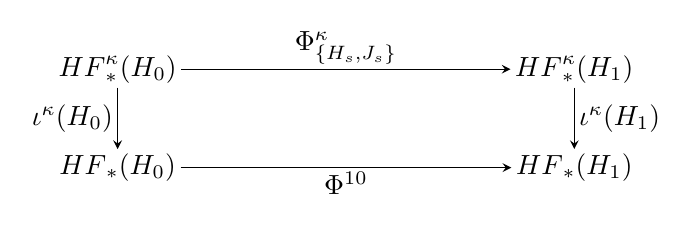
\begin{tikzpicture}[baseline=(current bounding box.center),>=stealth,
  every node/.style={inner sep=1.5pt}]
  \node (a) at (0,1.25) {$\operatorname{HF}_*^\kappa(H_0)$};
  \node (b) at (5.8,1.25) {$\operatorname{HF}_*^\kappa(H_1)$};
  \node (c) at (0,0) {$\operatorname{HF}_*(H_0)$};
  \node (d) at (5.8,0) {$\operatorname{HF}_*(H_1)$};
  \draw[->] (a) -- node[above] {$\Phi^\kappa_{\{H_s,J_s\}}$} (b);
  \draw[->] (a) -- node[left] {$\iota^\kappa(H_0)$} (c);
  \draw[->] (b) -- node[right] {$\iota^\kappa(H_1)$} (d);
  \draw[->] (c) -- node[below] {$\Phi^{10}$} (d);
\end{tikzpicture}
\end{equation}
其中 $\Phi^\kappa_{\{H_s,J_s\}}$ 是\BookRecordIndex{T0240}滤过弗洛尔同调的延拓同构，$\Phi^{10}$ 是典范的
弗洛尔延拓同构。

\paragraph{\BookRecordIndex{T0271}谱不变量。}
\BookRecordIndex{T0240}滤过弗洛尔同调群给出函数
\[
  \rho:\widetilde{\operatorname{Ham}}(M,\omega)
  \times\operatorname{QH}^*(M;\Lambda_\omega)
  \longrightarrow\mathbb R\cup\{-\infty\},
\]
定义为
\begin{equation}\label{eq:12-4-3}
  \rho(\widetilde\phi^H;a)
  :=\inf\bigl\{\kappa\in\mathbb R\setminus\operatorname{Spec}(H)
  \bigm|\Phi_*^{\mathrm{PSS}}(\operatorname{PD}(a))
  \in\operatorname{im}\iota^\kappa(H)\bigr\}.
\end{equation}
这里
\[
  \Phi_*^{\mathrm{PSS}}:
  \operatorname{QH}_*(M;\check\Lambda)
  \longrightarrow\operatorname{HF}_*(H)
\]
表示哈密顿函数 $H$ 的 PSS 同构，而
\[
  \operatorname{PD}:\operatorname{QH}^*(M;\Lambda_\omega)
  \longrightarrow\operatorname{QH}_*(M;\check\Lambda_\omega)
\]
表示注~\ref{rem:11-1-20} 定义的 Poincaré 对偶同构。交换图~\eqref{eq:12-4-2}
表明，数 $\rho(\widetilde\phi;a)$ 与定义它时所用的、满足
$\widetilde\phi^H=\widetilde\phi$ 的哈密顿函数 $H$ 无关。它称为
$\widetilde\phi\in\widetilde{\operatorname{Ham}}(M,\omega)$ 与
$a\in\operatorname{QH}^*(M;\Lambda_\omega)$ 的\emph{\BookRecordIndex{T0271}谱不变量}。

为从几何上理解 $\rho(\widetilde\phi;a)$，假定存在\BookRecordIndex{T0406}正则对 $(H,J)$，使得
$\widetilde\phi=\widetilde\phi^H$。再设
\[
  a=\sum_Aa_A\otimes e^A
  \in\operatorname{QH}^{2n-k}(M;\Lambda_\omega),
\]
其中 $a_A\in H^{2n-k-2c_1(A)}(M)$，并假定每个 $a_A$ 都是定向子流形
$X_A\subset M$（维数为 $k+2c_1(A)$）的基本循环的 Poincaré 对偶。那么 $a$ 的
Poincaré 对偶是\BookRecordIndex{T0230}量子同调类
\[
  \operatorname{PD}(a)=\sum_A[X_A]\otimes e^{-A}
  \in\operatorname{QH}_k(M;\check\Lambda_\omega).
\]
它在 PSS 同构
\[
  \Phi_*^{\mathrm{PSS}}:\operatorname{QH}_k(M;\check\Lambda_\omega)
  \longrightarrow\operatorname{HF}_{k-n}(H,J)
\]
下的像，是链 $\eta:\widetilde{\mathcal P}(H)\to\mathbb Z$ 的\BookRecordIndex{T0132}弗洛尔同调类，其中
\begin{equation}\label{eq:12-4-4}
  \eta(\widetilde y):=\sum_A n\bigl(X_A,(-A)\#\widetilde y\bigr).
\end{equation}
这里 $n(X,\widetilde x)$ 表示满足 $u(0)\in X$、如图~\ref{fig:12-1-1} 所示的\BookRecordIndex{T0182}尖盘
$u\in\mathcal M(\widetilde x;H,J)$ 的带符号计数。注意，数
$n(X_A,(-A)\#\widetilde y)$ 只有在
\[
\begin{aligned}
  n-\mu_{\mathrm{CZ}}(\widetilde y)-2c_1(A)
  &=\dim\mathcal M((-A)\#\widetilde y;H,J)\\
  &=\operatorname{codim}X_A\\
  &=2n-k-2c_1(A)
\end{aligned}
\]
时才可能非零，等价地，$\mu_{\mathrm{CZ}}(\widetilde y)=k-n$。因此，如所预期，
$\eta$ 的\BookRecordIndex{T0132}弗洛尔同调类属于 $\operatorname{HF}_{k-n}(H,J)$。条件
$\kappa\ge\rho(\widetilde\phi^H;a)$ 等价于存在弗洛尔链
$\eta'\in\operatorname{CF}_{k-n}^\kappa(H)$ 和
$\zeta\in\operatorname{CF}_{k-n+1}(H)$，使得 $\eta=\eta'+\partial\zeta$。

\begin{exercise}\label{ex:12-4-3}
证明在交换图~\eqref{eq:12-4-2} 中，只要 $\kappa<\kappa'$，
$\iota^\kappa(H)$ 的像就包含于 $\iota^{\kappa'}(H)$ 的像。因此把
$\rho(\widetilde\phi;a)$ 刻画为 $\operatorname{Spec}(\widetilde\phi)$ 中唯一满足如下
条件的元素：当 $\kappa>\rho(\widetilde\phi;a)$ 时，
$\Phi_*^{\mathrm{PSS}}(\operatorname{PD}(a))\in\operatorname{im}\iota^\kappa(H)$；当
$\kappa<\rho(\widetilde\phi;a)$ 时，
$\Phi_*^{\mathrm{PSS}}(\operatorname{PD}(a))\notin\operatorname{im}\iota^\kappa(H)$。
\end{exercise}

\begin{theorem}[Oh]\label{thm:12-4-4}
设 $(M,\omega)$ 是满足~\eqref{eq:8-5-1} 和~\eqref{eq:12-4-1} 的闭\BookRecordIndex{T0358}辛流形。则下列各项
成立。

\begin{description}
\item[（谱性）] 若 $a\ne0$，则对每个
$\widetilde\phi\in\widetilde{\operatorname{Ham}}(M,\omega)$ 都有
\[
  \rho(\widetilde\phi;a)\in\operatorname{Spec}(\widetilde\phi).
\]

\item[（辛不变性）] 对所有 $\psi\in\operatorname{Symp}(M,\omega)$、
$\widetilde\phi\in\widetilde{\operatorname{Ham}}(M,\omega)$ 以及
$a\in\operatorname{QH}^*(M;\Lambda)$，都有
\[
  \rho(\psi\widetilde\phi\psi^{-1};a)=\rho(\widetilde\phi;a).
\]
\sourcefootnote{原书对任意 $\psi\in\operatorname{Symp}(M,\omega)$ 固定 $a$ 写出此式；
一般的自然性公式还应同时施加 $\psi$ 在\BookRecordIndex{T0229}量子上同调上诱导的作用。因此，原式固定 $a$ 的
版本至少还需假定 $a$ 在该作用下不变；特别地，对
$\psi\in\operatorname{Symp}_0(M,\omega)$（包括下文实际使用的哈密顿情形）这一条件成立。}

\item[（连续性）] 若 $a\ne0$，则映射
\[
  \widetilde{\operatorname{Ham}}(M,\omega)\longrightarrow\mathbb R,
  \qquad \widetilde\phi\longmapsto\rho(\widetilde\phi;a)
\]
关于 $\widetilde{\operatorname{Ham}}(M,\omega)$ 上的 \BookRecordIndex{T0027}Hofer 度量连续。更准确地说，若
$a\ne0$，而 $H_0,H_1\in\mathcal H$ 是分别生成
$\widetilde\phi_0,\widetilde\phi_1\in
\widetilde{\operatorname{Ham}}(M,\omega)$ 的哈密顿函数，则
\begin{equation}\label{eq:12-4-5}
  \int_0^1\min_M(H_{1,t}-H_{0,t})\,dt
  \le\rho(\widetilde\phi_0;a)-\rho(\widetilde\phi_1;a)
  \le\int_0^1\max_M(H_{1,t}-H_{0,t})\,dt.
\end{equation}

\item[（零元）] 若 $0\ne a\in H^*(M)$ 且 $A\in H_2^S(M)$，则
\[
  \rho(\operatorname{id};a\otimes e^A)=\omega(A).
\]

\item[（乘积）] 对所有
$\widetilde\phi,\widetilde\psi\in\widetilde{\operatorname{Ham}}(M,\omega)$ 以及
$a,b\in\operatorname{QH}^*(M;\Lambda_\omega)$，都有
\[
  \rho(\widetilde\phi\widetilde\psi;a*b)
  \le\rho(\widetilde\phi;a)+\rho(\widetilde\psi;b).
\]

\item[（非退化性）] 对每个满足 $\phi\ne\operatorname{id}$ 的
$\phi\in\operatorname{Ham}(M,\omega)$，都存在常数 $\delta>0$，使得对每个
$H\in\mathcal H(M,\omega)$ 都有
\[
  \phi^H=\phi\qquad\Longrightarrow\qquad
  \rho(\widetilde\phi^H;1)+\rho((\widetilde\phi^H)^{-1};1)\ge\delta.
\]
\end{description}
\end{theorem}

\begin{proof}
我们略去“乘积”公理的证明；它本质上与 Schwarz \srcite{360} 给出的证明相同。在
假设~\eqref{eq:12-4-1} 下，我们概述其余公理的证明。一般情形参见 Usher
\srcite{398}。

由定义，每个\BookRecordIndex{T0132}弗洛尔同调类都属于某个 $\kappa$ 所对应映射
\[
  \iota^\kappa(H):\operatorname{HF}_*^\kappa(H,J)
  \longrightarrow\operatorname{HF}_*(H,J)
\]
的像。因此，对每个 $a$ 都有 $\rho(\widetilde\phi;a)<\infty$。若 $a\ne0$，则
$\Phi_*^{\mathrm{PSS}}(\operatorname{PD}(a))$ 非零，因而不可能对每个 $\kappa$ 都属于
$\iota^\kappa(H)$ 的像。（由下面的习题~\ref{ex:12-4-6}，这些像的交为零。）这表明，只要
$a\ne0$，$\rho(\widetilde\phi;a)$ 就是实数。这个数属于
$\widetilde\phi$ 的谱，是因为同态 $\iota^\kappa(H)$ 的像只有在 $\kappa$ 穿过
$\operatorname{Spec}(H)$ 中的元素时才可能改变。这证明了“谱性”公理。“辛不变性”公理
直接由定义得到。

“连续性”公理的证明分两步。关于
$\widetilde{\operatorname{Ham}}(M,\omega)$ 上 $C^1$-范数的连续性来自\BookRecordIndex{T0240}滤过弗洛尔同调的
“同伦性”公理：若 $H\in\mathcal H^\kappa$，而 $H'$ 在 $C^2$-范数下充分接近 $H$，则
$H'\in\mathcal H^\kappa$；事实上，$H'$ 可在 $\mathcal H^\kappa$ 中沿一条道路与 $H$
同伦。因此由交换图~\eqref{eq:12-4-2}，弗洛尔延拓同态
$\operatorname{HF}_*(H)\to\operatorname{HF}_*(H')$ 在
$\operatorname{im}\iota^\kappa(H)$ 与 $\operatorname{im}\iota^\kappa(H')$ 之间诱导同构。
这证明了关于 $C^1$-范数的连续性。

为证明~\eqref{eq:12-4-5}，假定存在\BookRecordIndex{T0088}殆复结构 $J_0,J_1\in\mathcal J$，使得
$(H_0,J_0)$ 与 $(H_1,J_1)$ 是\BookRecordIndex{T0132}弗洛尔同调的\BookRecordIndex{T0406}正则对。再令
$\mathbb R\to\mathcal J:s\mapsto J_s$ 是一条光滑道路，它在 $s\le0$ 时等于 $J_0$，
在 $s\ge1$ 时等于 $J_1$。取光滑\BookRecordIndex{T0188}截断函数 $\beta:\mathbb R\to[0,1]$，满足
\[
  \beta(s)=
  \begin{cases}
    0,&s\le0,\\
    1,&s\ge1,
  \end{cases}
  \qquad \partial_s\beta\ge0,
\]
并定义 $H_{s,t}:M\to\mathbb R$ 为
\[
  H_{s,t}:=\beta(s)H_{1,t}+(1-\beta(s))H_{0,t}.
\]
先假定 $\{H_s,J_s\}$ 是\BookRecordIndex{T0132}弗洛尔同调的\BookRecordIndex{T0407}正则同伦。令
\[
  \kappa>\rho(\widetilde\phi_0;a).
\]
于是存在\BookRecordIndex{T0132}弗洛尔同调循环 $\eta_0\in\operatorname{CF}_*(H_0)$，它代表\BookRecordIndex{T0132}弗洛尔同调类
\[
  \alpha_0:=\Phi_*^{\mathrm{PSS}}(\operatorname{PD}(a))
  \in\operatorname{HF}_*(H_0,J_0),
\]
并且对每个 $\widetilde x_0\in\widetilde{\mathcal P}(H_0)$ 都满足
\[
  \eta_0(\widetilde x_0)\ne0
  \qquad\Longrightarrow\qquad
  \mathcal A_{H_0}(\widetilde x_0)\le\kappa.
\]
对具有相同 Conley--Zehnder 指数的
$\widetilde x_0\in\widetilde{\mathcal P}(H_0)$ 与
$\widetilde x_1\in\widetilde{\mathcal P}(H_1)$，用
$n(\widetilde x_0,\widetilde x_1)$ 表示从 $\widetilde x_0$ 连接到
$\widetilde x_1$ 的方程~\eqref{eq:12-1-10} 之解的带符号计数。定义
$\eta_1\in\operatorname{CF}_*(H_1)$ 为
\[
  \eta_1(\widetilde x_1)
  :=\sum_{\widetilde x_0\in\widetilde{\mathcal P}(H_0)}
  \eta_0(\widetilde x_0)n(\widetilde x_0,\widetilde x_1).
\]
于是 $\eta_1$ 是一个弗洛尔链，代表 $[\eta_0]$ 在弗洛尔延拓同构下的像，即\BookRecordIndex{T0132}弗洛尔同调类
\[
  \alpha_1:=\Phi_*^{\mathrm{PSS}}(\operatorname{PD}(a))
  \in\operatorname{HF}_*(H_1,J_1).
\]
现在，方程~\eqref{eq:12-1-10} 的解所满足的\BookRecordIndex{T0249}能量恒等式~\eqref{eq:12-1-11} 表明，
$n(\widetilde x_0,\widetilde x_1)$ 只有在
\[
\begin{aligned}
  \mathcal A_{H_0}(\widetilde x_0)-\mathcal A_{H_1}(\widetilde x_1)
  &\ge\int_{-\infty}^{\infty}\int_0^1
  \min_M\partial_sH_{s,t}\,dt\,ds\\
  &=\int_0^1\min_M(H_{1,t}-H_{0,t})\,dt
\end{aligned}
\]
时才可能非零。最后一个等号来自同伦 $H_{s,t}$ 的特殊形式。因此，若
$\eta_1(\widetilde x_1)\ne0$，则存在
$\widetilde x_0\in\widetilde{\mathcal P}(H_0)$，使得
$\eta_0(\widetilde x_0)\ne0$ 且
$n(\widetilde x_0,\widetilde x_1)\ne0$，从而
\[
  \mathcal A_{H_1}(\widetilde x_1)
  \le\mathcal A_{H_0}(\widetilde x_0)
  -\int_0^1\min_M(H_{1,t}-H_{0,t})\,dt
  \le\kappa-\int_0^1\min_M(H_{1,t}-H_{0,t})\,dt.
\]
因为 $\eta_1$ 代表\BookRecordIndex{T0132}弗洛尔同调类
$\Phi_*^{\mathrm{PSS}}(\operatorname{PD}(a))\in\operatorname{HF}_*(H_1,J_1)$，故
\[
  \rho(\widetilde\phi_1;a)
  \le\kappa-\int_0^1\min_M(H_{1,t}-H_{0,t})\,dt.
\]
对所有 $\kappa>\rho(\widetilde\phi_0;a)$ 取下确界，得到
\[
  \rho(\widetilde\phi_1;a)
  \le\rho(\widetilde\phi_0;a)
  -\int_0^1\min_M(H_{1,t}-H_{0,t})\,dt.
\]
这在 $\{H_s,J_s\}$ 是\BookRecordIndex{T0407}正则同伦的假设下证明了~\eqref{eq:12-4-5} 的第一个不等式。一般
情形下，在正则端点之间用\BookRecordIndex{T0407}正则同伦逼近 $(H_s,J_s)$，再利用已经证明的如下连续性：在
$\widetilde{\operatorname{Ham}}(M,\omega)$ 上关于 $C^1$-范数连续，相应地在哈密顿函数
空间上关于 $C^2$-范数连续。交换 $H_0$ 与 $H_1$，即可由第一个不等式得到
\eqref{eq:12-4-5} 的第二个不等式。

为证明“零元”公理，可以取一列正则哈密顿函数
$H_i\in\mathcal H(M,\omega)$，使其在 $C^\infty$ 拓扑中收敛到零。于是存在一列
$\varepsilon_i>0$，满足 $\varepsilon_i\to0$，而且下列经补正的包含式成立
\sourcefootnote{原书在中项把 $\iota^\kappa$ 的自变量误印为 $H$；但
$\Psi^{f,H_i}$ 的定义域是 $\operatorname{HF}_*(H_i)$，且本段使用的正则逼近列也是
$H_i$，故唯一应为 $\operatorname{im}\iota^\kappa(H_i)$。}：
\[
  \operatorname{im}\iota^{\kappa-\varepsilon_i}(f)
  \subset\Psi^{f,H_i}\bigl(\operatorname{im}\iota^\kappa(H_i)\bigr)
  \subset\operatorname{im}\iota^{\kappa+\varepsilon_i}(f).
\]
这里采用下面习题~\ref{ex:12-4-6} 的记号。换言之，可以构造这些 PSS 映射，使\BookRecordIndex{T0249}能量
恒等式~\eqref{eq:12-1-14} 中的常数 $c_E$ 任意小。由此可以证明，对每个非零上同调类
$a\in H^*(M)$，$\rho(\widetilde\phi^{H_i};a)$ 都收敛到零。因此，在 $A=0$ 的情形，
“零元”公理由“连续性”公理得出。为证明 $A\ne0$ 的结论，可以使用\BookRecordIndex{T0132}弗洛尔同调在 Novikov
环上的模结构。

下面概述如下事实的证明：对每个满足 $\phi\ne\operatorname{id}$ 的
$\phi\in\operatorname{Ham}(M,\omega)$，存在常数 $\delta>0$，使得对每个
$H\in\mathcal H(M,\omega)$ 都有
\begin{equation}\label{eq:12-4-6}
  \phi^H=\phi\qquad\Longrightarrow\qquad
  \rho(\widetilde\phi^H;1)
  -\rho(\widetilde\phi^H;\operatorname{PD}([\mathrm{pt}]))\ge\delta.
\end{equation}
“非退化性”公理由~\eqref{eq:12-4-6} 和“乘积”公理立即\BookRecordIndex{T0326}推出。事实上，若
$\phi^H=\phi$，则
\[
\begin{aligned}
  \rho(\widetilde\phi^H;1)+\rho((\widetilde\phi^H)^{-1};1)
  &\ge\rho(\widetilde\phi^H;1)
  -\rho(\widetilde\phi^H;\operatorname{PD}([\mathrm{pt}]))
  +\rho(\operatorname{id};\operatorname{PD}([\mathrm{pt}]))\\
  &\ge\delta.
\end{aligned}
\]
第一个不等式来自“乘积”公理，最后一个来自“零元”公理与~\eqref{eq:12-4-6}。

为证明估计~\eqref{eq:12-4-6}，像推论~\ref{cor:9-1-14} 的证明那样定义常数
$\delta$：任取\BookRecordIndex{T0088}殆复结构的光滑族
$\mathbb R\to\mathcal J:t\mapsto\widetilde J_t$，满足
$\widetilde J_{t+1}=\phi^*\widetilde J_t$；取
$x_0\in M\setminus\operatorname{Fix}(\phi)$，对光滑函数
$\widetilde u:\mathbb R^2\to M$ 考虑方程
\begin{equation}\label{eq:12-4-7}
  \partial_s\widetilde u
  +\widetilde J_t(\widetilde u)\partial_t\widetilde u=0,
  \qquad
  \widetilde u(s,t)=\phi(\widetilde u(s,t+1)),
  \qquad
  \widetilde u(0,0)=x_0,
\end{equation}
并定义
\[
  \delta:=\min\bigl\{\min_t\hbar(\widetilde J_t),\delta_0\bigr\},
  \qquad
  \delta_0:=\inf\bigl\{E(\widetilde u)\bigm|
  \widetilde u\text{ 满足~\eqref{eq:12-4-7}},\ E(\widetilde u)<\infty\bigr\}.
\]
这里 $\hbar(\widetilde J_t)$ 表示非常值 $\widetilde J_t$-全纯球面的最小面积。由
命题~\ref{prop:4-1-4} 以及
$\hbar(\widetilde J_{t+1})=\hbar(\widetilde J_t)$，数
$\min_t\hbar(\widetilde J_t)$ 为正。数 $\delta_0$ 的正性来自一个显然的\BookRecordIndex{T0192}紧性论证：若
$\widetilde u_i$ 是~\eqref{eq:12-4-7} 的解且 $E(\widetilde u_i)\to0$，则有一个子列在
紧集上连同所有导数一致收敛到~\eqref{eq:12-4-7} 的解 $\widetilde u$，且
$E(\widetilde u)=0$；任意这样的解都必须形如
$\widetilde u(s,t)\equiv x_0=\phi(x_0)$，这与 $x_0$ 不是 $\phi$ 的不动点矛盾。因此
$\delta>0$。下面证明的一个推论是 $\delta<\infty$；这一点从定义并不明显。（另一种证明
见定理~\ref{thm:9-1-13}。）

取满足 $\phi^H=\phi$ 的 $H\in\mathcal H$，用 $\phi_t$ 表示 $H$ 确定的\BookRecordIndex{T0158}哈密顿同痕，
并由公式 $\phi_t^*J_t:=\widetilde J_t$ 定义 $J_t=J_{t+1}\in\mathcal J$。我们先在如下
假设下证明~\eqref{eq:12-4-6}：$(H,J)$ 是\BookRecordIndex{T0132}弗洛尔同调以及上面所选点 $x_0$ 的\BookRecordIndex{T0406}正则对。
在这个假设下，存在算子
\[
  \Psi_0:\operatorname{HF}_n(H,J)\longrightarrow\operatorname{HF}_{-n}(H,J),
\]
其定义为
\[
  (\Psi_0\eta)(\widetilde y)
  :=\sum_{\mu_{\mathrm{CZ}}(\widetilde x)=n}
  \eta(\widetilde x)n_H(\widetilde x,\widetilde y;x_0),
\]
其中 $n_H(\widetilde x,\widetilde y;x_0)$ 表示从 $\widetilde x$ 到 $\widetilde y$、通过
$x_0$ 的\BookRecordIndex{T0131}弗洛尔连接轨道的带符号计数。因此，
$n_H(\widetilde x,\widetilde y;x_0)$ 计数方程
\begin{equation}\label{eq:12-4-8}
  \partial_su+J_t(u)(\partial_tu-X_{H_t}(u))=0,
  \qquad u(s,t)=u(s,t+1),
  \qquad u(0,0)=x_0
\end{equation}
的解。正如注~\ref{rem:12-3-3} 指出的，
\begin{equation}\label{eq:12-4-9}
  \Psi_0\circ\Phi_*^{\mathrm{PSS}}([M])
  =\Phi_*^{\mathrm{PSS}}([\mathrm{pt}]).
\end{equation}
现在任取实数 $\kappa$，使得
\[
  \kappa\notin\operatorname{Spec}(\widetilde\phi^H),
  \qquad \rho(\widetilde\phi^H;1)<\kappa.
\]
于是存在\BookRecordIndex{T0132}弗洛尔同调循环 $\eta_1\in\operatorname{CF}_n(H)$，满足
$[\eta_1]=\Phi_*^{\mathrm{PSS}}([M])$，并且对每个
$\widetilde x\in\widetilde{\mathcal P}(H)$ 都有
\begin{equation}\label{eq:12-4-10}
  \mathcal A_H(\widetilde x)>\kappa
  \qquad\Longrightarrow\qquad \eta_1(\widetilde x)=0.
\end{equation}
定义 $\eta_0\in\operatorname{CF}_{-n}(H)$ 为
\[
  \eta_0(\widetilde y)
  :=\sum_{\mu_{\mathrm{CZ}}(\widetilde x)=n}
  \eta_1(\widetilde x)n_H(\widetilde x,\widetilde y;x_0).
\]
由~\eqref{eq:12-4-9}，$\eta_0$ 是\BookRecordIndex{T0132}弗洛尔同调循环，且
$[\eta_0]=\Phi_*^{\mathrm{PSS}}([\mathrm{pt}])$。此外，
\[
  \mathcal A_H(\widetilde y)>\kappa-\delta
  \qquad\Longrightarrow\qquad\eta_0(\widetilde y)=0.
\]
为看出这一点，注意~\eqref{eq:12-4-8} 的每个解 $u$ 都等价于
\eqref{eq:12-4-7} 的解
\[
  \widetilde u(s,t):=\phi_t^{-1}(u(s,t)),
\]
因而 $E(u)\ge\delta$。这说明，$\Psi_0(\eta_1)$ 定义中的系数
$n_H(\widetilde x,\widetilde y;x_0)$ 只有在
\[
  \mathcal A_H(\widetilde x)-\mathcal A_H(\widetilde y)\ge\delta
\]
时才可能非零。因此由~\eqref{eq:12-4-10}，$\eta_0(\widetilde y)$ 只有在存在
$\widetilde x\in\widetilde{\mathcal P}(H)$，满足
$\mu_{\mathrm{CZ}}(\widetilde x)=n$、$\eta_1(\widetilde x)\ne0$ 且
\[
  \mathcal A_H(\widetilde y)
  \le\mathcal A_H(\widetilde x)-\delta\le\kappa-\delta
\]
时才可能非零。于是我们证明了\BookRecordIndex{T0132}弗洛尔同调类
$\Phi_*^{\mathrm{PSS}}([\mathrm{pt}])=[\eta_0]$ 属于同态
\[
  \iota^{\kappa-\delta}(H):
  \operatorname{HF}_{-n}^{\kappa-\delta}(H,J)
  \longrightarrow\operatorname{HF}_{-n}(H,J)
\]
的像，因而
\[
  \rho(\widetilde\phi^H;\operatorname{PD}([\mathrm{pt}]))
  \le\kappa-\delta.
\]
这就在 $(H,J)$ 是\BookRecordIndex{T0406}正则对的情形证明了不等式~\eqref{eq:12-4-6}。

为证明一般结论，取一列收敛到 $(H,J)$ 的\BookRecordIndex{T0406}正则对 $(H_i,J_i)$，并用 $\delta_i$ 表示把
上面的 $(\phi,\widetilde J_t)$ 换成 $(\phi_{i1},\phi_{it}^*J_{it})$ 后得到的同一常数；这里
$\phi_{it}$ 表示 $H_i$ 生成的\BookRecordIndex{T0158}哈密顿同痕。我们断言
\begin{equation}\label{eq:12-4-11}
  \liminf_{i\to\infty}\delta_i\ge\delta.
\end{equation}
为此，固定正实数 $\varepsilon<\delta$。必须证明当 $i$ 充分大时
$\varepsilon<\delta_i$。反设不然。必要时取子列，可假定对每个 $i$ 都有
$\delta_i\le\varepsilon$。若存在序列 $i_\nu\to\infty$，使得
$\min_t\hbar(J_{i_\nu t})\le\varepsilon$，则由于
$\phi_{i_\nu t}^*J_{i_\nu t}$ 收敛到 $\widetilde J_t$，由\BookRecordIndex{T0139}格罗莫夫紧性可知
$\min_t\hbar(\widetilde J_t)\le\varepsilon<\delta$，这与 $\delta$ 的定义矛盾。因此，当
$i$ 充分大时必须有 $\min_t\hbar(J_{it})>\varepsilon$。又因为
$\delta_i\le\varepsilon$，存在~\eqref{eq:12-4-7} 的一列解 $\widetilde u_i$（其中把
$\phi$ 换成 $\phi_{i1}$、把 $\widetilde J_t$ 换成 $\phi_{it}^*J_{it}$），使得
$E(\widetilde u_i)\le\varepsilon$。按假设，对每个 $t$ 都有
$\varepsilon<\hbar(\widetilde J_t)$，故不能发生\BookRecordIndex{T0243}冒泡；于是 $\widetilde u_i$ 有一个子列
收敛到~\eqref{eq:12-4-7} 的解 $\widetilde u$。从而
$E(\widetilde u)\le\varepsilon<\delta$，再次与 $\delta$ 的定义矛盾。这就证明了
\eqref{eq:12-4-11}。

由已经证明的特殊情形，对每个 $i$ 都有
\[
  \rho(\widetilde\phi^{H_i};1)
  -\rho(\widetilde\phi^{H_i};\operatorname{PD}([\mathrm{pt}]))
  \ge\delta_i.
\]
令 $i\to\infty$ 并使用~\eqref{eq:12-4-11}，即得估计~\eqref{eq:12-4-6}。
\end{proof}

注意，一般而言，\BookRecordIndex{T0027}Hofer 度量在
$\widetilde{\operatorname{Ham}}(M,\omega)$ 上未必诱导出一个度量：当且仅当哈密顿环路的
每个非平凡同伦类都有正的最小 Hofer 长度时，它才诱导出度量。目前还没有发现支持最小
长度为零的不可缩环路的闭流形。若这样的环路确实存在，则“连续性”公理表明\BookRecordIndex{T0271}谱不变量下降到
$\operatorname{Ham}(M,\omega)$ 的一个更小覆叠空间。

$\rho$ 的“乘积”公理可以解释为\BookRecordIndex{T0271}谱不变量与量子乘法之间的\BookRecordIndex{T0348}相容性。Schwarz
\srcite{360} 首先在\BookRecordIndex{T0355}辛非球面情形注意到这一性质。所有最有趣的应用都以它为基础，例如用
\BookRecordIndex{T0271}谱不变量定义 \BookRecordIndex{T0028}Hofer 范数的类似物（见 Viterbo \srcite{404}、Schwarz \srcite{360}
和 Oh \srcite{307}），以及 Entov--Polterovich 在 \srcite{105} 中构造 Calabi \BookRecordIndex{T0253}拟同态。
这里不尝试解释这些应用。不过，在下面的引理~\ref{lem:12-5-3} 中，我们会描述群
$\pi_1(\operatorname{Ham}(M,\omega))$ 的一个扩张在\BookRecordIndex{T0271}谱不变量上的作用。

\begin{remark}\label{rem:12-4-5}
定理~\ref{thm:12-4-4} 的“辛不变性”公理可以改述为
\[
  \rho(\widetilde\phi\widetilde\psi;a)
  =\rho(\widetilde\psi\widetilde\phi;a)
\]
对所有 $\widetilde\phi,\widetilde\psi\in
\widetilde{\operatorname{Ham}}(M,\omega)$ 成立。为此，回忆习题~\ref{ex:12-4-2}：只要
$\widetilde\psi$ 是 $\psi$ 的提升，就有
$\widetilde\psi\widetilde\phi\widetilde\psi^{-1}
=\psi\widetilde\phi\psi^{-1}$ 于
$\widetilde{\operatorname{Ham}}(M,\omega)$ 中成立。
\end{remark}

\begin{exercise}\label{ex:12-4-6}
证明
\[
  \bigcap_\kappa\operatorname{im}\iota^\kappa(H)=\{0\}.
\]
\BookRecordIndex{T0326}推出对所有 $a\ne0$ 的 $(\widetilde\phi,a)$ 都有
$\rho(\widetilde\phi;a)>-\infty$。

\emph{提示：}以 Novikov 环为系数定义类似的\BookRecordIndex{T0239}滤过 Morse 同调群，并考虑同态
\[
  \iota^\kappa(f):\operatorname{HM}_*^\kappa(f;\Lambda_\omega)
  \longrightarrow\operatorname{HM}_*(f;\Lambda_\omega).
\]
证明
\[
  \bigcap_\kappa\operatorname{im}\iota^\kappa(f)=\{0\}.
\]
现在令
\[
  \Psi^{f,H}:\operatorname{HF}_*(H,J)
  \longrightarrow\operatorname{HM}_*(f;\Lambda_\omega)
\]
为 PSS 同构。利用\BookRecordIndex{T0249}能量恒等式~\eqref{eq:12-1-14} 证明：存在常数 $c>0$，使得对每个
$\kappa\in\mathbb R$ 都有
\[
  \Psi^{f,H}\bigl(\operatorname{im}\iota^\kappa(H)\bigr)
  \subset\operatorname{im}\iota^{\kappa+c}(f).
\]
然后利用如下事实：$\Psi^{f,H}$ 是同构
$\operatorname{QH}_*(M;\check\Lambda)\to
\operatorname{HM}_*(f;\Lambda_\omega)$ 与
$(\Phi_*^{\mathrm{PSS}})^{-1}$ 的复合。
\end{exercise}

\begin{exercise}\label{ex:12-4-7}
对 $\kappa\in(\mathbb R\setminus\operatorname{Spec}(H))\cup\{-\infty\}$，定义\BookRecordIndex{T0239}滤过上链群
\[
  \operatorname{CF}^*_\kappa(H)
  :=\bigl\{\xi\in\operatorname{CF}^*(H)\bigm|
  \xi(\widetilde x)\ne0\Longrightarrow
  \mathcal A_H(\widetilde x)\ge\kappa\bigr\}.
\]
验证弗洛尔上边缘算子 $\delta$ 把 $\operatorname{CF}^*_\kappa(H)$ 映入自身，并由此对
$H\in\mathcal H^\kappa$ 定义\BookRecordIndex{T0239}滤过弗洛尔上同调群
$\operatorname{HF}^*_\kappa(H)$。用
\[
  j_\kappa(H):\operatorname{HF}^*_\kappa(H)
  \longrightarrow\operatorname{QH}^*(M;\Lambda_\omega)
\]
表示同态 $\operatorname{HF}^*_\kappa(H,J)\to\operatorname{HF}^*(H,J)$ 与 PSS 同构
$\operatorname{HF}^*(H,J)\to\operatorname{QH}^*(M;\Lambda_\omega)$ 的复合。证明对每个
$a\in\operatorname{QH}^*(M;\Lambda_\omega)$ 都有
\begin{equation}\label{eq:12-4-12}
  \rho((\widetilde\phi^H)^{-1};a)
  =-\sup\bigl\{\kappa\in\mathbb R\setminus\operatorname{Spec}(H)
  \bigm|a\in\operatorname{im}j_\kappa(H)\bigr\}.
\end{equation}
\end{exercise}

\begin{exercise}\label{ex:12-4-8}
利用定理~\ref{thm:12-4-4} 证明
\[
  d(\phi,\psi)
  :=\inf_{\phi^H=\phi\psi^{-1}}
  \left(\rho(\widetilde\phi^H;1)
  +\rho((\widetilde\phi^H)^{-1};1)\right)
\]
是 $\operatorname{Ham}(M,\omega)$ 上的度量。
\end{exercise}
